% Copyright © 2013 Martin Ueding <dev@martin-ueding.de>

% Copyright © 2012-2013 Martin Ueding <dev@martin-ueding.de>

% This is my general purpose LaTeX header file for writing German documents.
% Ideally, you include this using a simple ``% Copyright © 2012-2013 Martin Ueding <dev@martin-ueding.de>

% This is my general purpose LaTeX header file for writing German documents.
% Ideally, you include this using a simple ``% Copyright © 2012-2013 Martin Ueding <dev@martin-ueding.de>

% This is my general purpose LaTeX header file for writing German documents.
% Ideally, you include this using a simple ``\input{header.tex}`` in your main
% document and start with ``\title`` and ``\begin{document}`` afterwards.

% If you need to add additional packages, I recommend not doing this in this
% file, but in your main document. That way, you can just drop in a new
% ``header.tex`` and get all the new commands without having to merge manually.

% Since this file encorporates a CC-BY-SA fragment, this whole files is
% licensed under the CC-BY-SA license.

\documentclass[11pt, ngerman, fleqn, DIV=15, BCOR=2cm, headinclude]{scrartcl}

\usepackage{graphicx}

% Environment to quote the problem. Currently, this is just a new name for the
% quote environment.
\newenvironment{problem}{\begin{quote}\textsf{\textbf{Aufgabenstellung:}}\quad}{\end{quote}}

\setkomafont{caption}{\sf}
\setkomafont{captionlabel}{\usekomafont{caption}}

%%%%%%%%%%%%%%%%%%%%%%%%%%%%%%%%%%%%%%%%%%%%%%%%%%%%%%%%%%%%%%%%%%%%%%%%%%%%%%%
%                                Locale, date                                 %
%%%%%%%%%%%%%%%%%%%%%%%%%%%%%%%%%%%%%%%%%%%%%%%%%%%%%%%%%%%%%%%%%%%%%%%%%%%%%%%

\usepackage{babel}
\usepackage[iso]{isodate}

%%%%%%%%%%%%%%%%%%%%%%%%%%%%%%%%%%%%%%%%%%%%%%%%%%%%%%%%%%%%%%%%%%%%%%%%%%%%%%%
%                          Margins and other spacing                          %
%%%%%%%%%%%%%%%%%%%%%%%%%%%%%%%%%%%%%%%%%%%%%%%%%%%%%%%%%%%%%%%%%%%%%%%%%%%%%%%

\usepackage[parfill]{parskip}
\usepackage{setspace}
\usepackage[activate]{microtype}

\setlength{\columnsep}{2cm}

%%%%%%%%%%%%%%%%%%%%%%%%%%%%%%%%%%%%%%%%%%%%%%%%%%%%%%%%%%%%%%%%%%%%%%%%%%%%%%%
%                                    Color                                    %
%%%%%%%%%%%%%%%%%%%%%%%%%%%%%%%%%%%%%%%%%%%%%%%%%%%%%%%%%%%%%%%%%%%%%%%%%%%%%%%

\usepackage[usenames, dvipsnames]{xcolor}

\colorlet{darkred}{red!70!black}
\colorlet{darkblue}{blue!70!black}
\colorlet{darkgreen}{green!40!black}

%%%%%%%%%%%%%%%%%%%%%%%%%%%%%%%%%%%%%%%%%%%%%%%%%%%%%%%%%%%%%%%%%%%%%%%%%%%%%%%
%                         Font and font like settings                         %
%%%%%%%%%%%%%%%%%%%%%%%%%%%%%%%%%%%%%%%%%%%%%%%%%%%%%%%%%%%%%%%%%%%%%%%%%%%%%%%

% This replaces all fonts with Bitstream Charter, Bitstream Vera Sans and
% Bitstream Vera Mono. Math will be rendered in Charter.
\usepackage[charter, greekuppercase=italicized]{mathdesign}
\usepackage{beramono}
\usepackage{berasans}

% Bold, sans-serif tensors. This fragment is taken from “egreg” from
% http://tex.stackexchange.com/a/82747/8945 and licensed under `CC-BY-SA
% <https://creativecommons.org/licenses/by-sa/3.0/>`_.
\usepackage{bm}
\DeclareMathAlphabet{\mathsfit}{\encodingdefault}{\sfdefault}{m}{sl}
\SetMathAlphabet{\mathsfit}{bold}{\encodingdefault}{\sfdefault}{bx}{sl}
\newcommand{\tens}[1]{\bm{\mathsfit{#1}}}

% Bold vectors.
\renewcommand{\vec}[1]{\boldsymbol{#1}}

%%%%%%%%%%%%%%%%%%%%%%%%%%%%%%%%%%%%%%%%%%%%%%%%%%%%%%%%%%%%%%%%%%%%%%%%%%%%%%%
%                               Input encoding                                %
%%%%%%%%%%%%%%%%%%%%%%%%%%%%%%%%%%%%%%%%%%%%%%%%%%%%%%%%%%%%%%%%%%%%%%%%%%%%%%%

\usepackage[T1]{fontenc}
\usepackage[utf8]{inputenc}

%%%%%%%%%%%%%%%%%%%%%%%%%%%%%%%%%%%%%%%%%%%%%%%%%%%%%%%%%%%%%%%%%%%%%%%%%%%%%%%
%                         Hyperrefs and PDF metadata                          %
%%%%%%%%%%%%%%%%%%%%%%%%%%%%%%%%%%%%%%%%%%%%%%%%%%%%%%%%%%%%%%%%%%%%%%%%%%%%%%%

\usepackage{hyperref}
\usepackage{lastpage}

% This sets the author in the properties of the PDF as well. If you want to
% change it, just override it with another ``\hypersetup`` call.
\hypersetup{
	breaklinks=false,
	citecolor=darkgreen,
	colorlinks=true,
	linkcolor=darkblue,
	menucolor=black,
	pdfauthor={Martin Ueding},
	urlcolor=darkblue,
}

%%%%%%%%%%%%%%%%%%%%%%%%%%%%%%%%%%%%%%%%%%%%%%%%%%%%%%%%%%%%%%%%%%%%%%%%%%%%%%%
%                               Math Operators                                %
%%%%%%%%%%%%%%%%%%%%%%%%%%%%%%%%%%%%%%%%%%%%%%%%%%%%%%%%%%%%%%%%%%%%%%%%%%%%%%%

% AMS environments like ``align`` and theorems like ``proof``.
\usepackage{amsmath}
\usepackage{amsthm}

% Common math constructs like partial derivatives.
\usepackage{commath}

% Physical units.
\usepackage[output-decimal-marker={,}]{siunitx}

% Since I use mathdesign with italic uppercase greek characters, the Ohm unit will be displayed with an italic Ω by default. Units have to be roman, so this forces it the right way.
\DeclareSIUnit{\ohm}{$\Omegaup$}
\DeclareSIUnit{\division}{DIV}
\DeclareSIUnit{\voltss}{$\mathrm{V_{SS}}$}

% Word like operators.
\DeclareMathOperator{\acosh}{arcosh}
\DeclareMathOperator{\arcosh}{arcosh}
\DeclareMathOperator{\arcsinh}{arsinh}
\DeclareMathOperator{\arsinh}{arsinh}
\DeclareMathOperator{\asinh}{arsinh}
\DeclareMathOperator{\card}{card}
\DeclareMathOperator{\csch}{cshs}
\DeclareMathOperator{\diam}{diam}
\DeclareMathOperator{\sech}{sech}
\renewcommand{\Im}{\mathop{{}\mathrm{Im}}\nolimits}
\renewcommand{\Re}{\mathop{{}\mathrm{Re}}\nolimits}

% Fourier transform.
\DeclareMathOperator{\fourier}{\ensuremath{\mathcal{F}}}

% Roman versions of “e” and “i” to serve as Euler's number and the imaginary
% constant.
\newcommand{\ee}{\eup}
\newcommand{\eup}{\mathrm e}
\newcommand{\ii}{\iup}
\newcommand{\iup}{\mathrm i}

% Symbols for the various mathematical fields (natural numbers, integers,
% rational numbers, real numbers, complex numbers).
\newcommand{\C}{\ensuremath{\mathbb C}}
\newcommand{\N}{\ensuremath{\mathbb N}}
\newcommand{\Q}{\ensuremath{\mathbb Q}}
\newcommand{\R}{\ensuremath{\mathbb R}}
\newcommand{\Z}{\ensuremath{\mathbb Z}}

% Shape like operators.
\DeclareMathOperator{\dalambert}{\Box}
\DeclareMathOperator{\laplace}{\bigtriangleup}
\newcommand{\curl}{\vnabla \times}
\newcommand{\divergence}[1]{\inner{\vnabla}{#1}}
\newcommand{\vnabla}{\vec \nabla}

\newcommand{\half}{\frac 12}

% Unit vector (German „Einheitsvektor“).
\newcommand{\ev}{\hat{\vec e}}

% Scientific notation for large numbers.
\newcommand{\e}[1]{\cdot 10^{#1}}

% Mathematician's notation for the inner (scalar, dot) product.
\newcommand{\bracket}[1]{\left\langle #1 \right\rangle}
\newcommand{\inner}[2]{\bracket{#1, #2}}

% Placeholders.
\newcommand{\emesswert}{\del{\messwert \pm \messwert}}
\newcommand{\fehlt}{\textcolor{darkred}{Hier fehlen noch Inhalte.}}
\newcommand{\messwert}{\textcolor{blue}{\square}}
\newcommand{\punkte}{\phantom{xxxxx}}
\newcommand{\punktevon}[1]{\begin{flushright}/ #1\end{flushright}}

% Separator for equations on a single line.
\newcommand{\eqnsep}{,\quad}

% Quantum Mechanics
\usepackage{braket}

%%%%%%%%%%%%%%%%%%%%%%%%%%%%%%%%%%%%%%%%%%%%%%%%%%%%%%%%%%%%%%%%%%%%%%%%%%%%%%%
%                                  Headings                                   %
%%%%%%%%%%%%%%%%%%%%%%%%%%%%%%%%%%%%%%%%%%%%%%%%%%%%%%%%%%%%%%%%%%%%%%%%%%%%%%%

% This will set fancy headings to the top of the page. The page number will be
% accompanied by the total number of pages. That way, you will know if any page
% is missing.
%
% If you do not want this for your document, you can just use
% ``\pagestyle{plain}``.

\usepackage{scrpage2}

\pagestyle{scrheadings}
\automark{section}
\cfoot{\footnotesize{Seite \thepage\ / \pageref{LastPage}}}
\chead{}
\ihead{}
\ohead{\rightmark}
\setheadsepline{.4pt}

%%%%%%%%%%%%%%%%%%%%%%%%%%%%%%%%%%%%%%%%%%%%%%%%%%%%%%%%%%%%%%%%%%%%%%%%%%%%%%%
%                            Bibliography (BibTeX)                            %
%%%%%%%%%%%%%%%%%%%%%%%%%%%%%%%%%%%%%%%%%%%%%%%%%%%%%%%%%%%%%%%%%%%%%%%%%%%%%%%

\newcommand{\bibliographyfile}{../../central-bibtex/Central}
\bibliographystyle{apalike2}

%%%%%%%%%%%%%%%%%%%%%%%%%%%%%%%%%%%%%%%%%%%%%%%%%%%%%%%%%%%%%%%%%%%%%%%%%%%%%%%
%                                Abbreviations                                %
%%%%%%%%%%%%%%%%%%%%%%%%%%%%%%%%%%%%%%%%%%%%%%%%%%%%%%%%%%%%%%%%%%%%%%%%%%%%%%%

\newcommand{\dhabk}{\mbox{d.\,h.}}

%%%%%%%%%%%%%%%%%%%%%%%%%%%%%%%%%%%%%%%%%%%%%%%%%%%%%%%%%%%%%%%%%%%%%%%%%%%%%%%
%                                  Licences                                   %
%%%%%%%%%%%%%%%%%%%%%%%%%%%%%%%%%%%%%%%%%%%%%%%%%%%%%%%%%%%%%%%%%%%%%%%%%%%%%%%

\usepackage{ccicons}

\newcommand{\ccbysadetext}{%
	\begin{small}
		Dieses Werk bzw. Inhalt steht unter einer
		\href{http://creativecommons.org/licenses/by-sa/3.0/deed.de}{%
			Creative Commons Namensnennung - Weitergabe unter gleichen
		Bedingungen 3.0 Unported Lizenz}.
	\end{small}
}

\newcommand{\ccbysadetitle}{%
	Lizenz: \href{http://creativecommons.org/licenses/by-sa/3.0/deed.de}
	{CC-BY-SA 3.0 \ccbysa}
}
`` in your main
% document and start with ``\title`` and ``\begin{document}`` afterwards.

% If you need to add additional packages, I recommend not doing this in this
% file, but in your main document. That way, you can just drop in a new
% ``header.tex`` and get all the new commands without having to merge manually.

% Since this file encorporates a CC-BY-SA fragment, this whole files is
% licensed under the CC-BY-SA license.

\documentclass[11pt, ngerman, fleqn, DIV=15, BCOR=2cm, headinclude]{scrartcl}

\usepackage{graphicx}

% Environment to quote the problem. Currently, this is just a new name for the
% quote environment.
\newenvironment{problem}{\begin{quote}\textsf{\textbf{Aufgabenstellung:}}\quad}{\end{quote}}

\setkomafont{caption}{\sf}
\setkomafont{captionlabel}{\usekomafont{caption}}

%%%%%%%%%%%%%%%%%%%%%%%%%%%%%%%%%%%%%%%%%%%%%%%%%%%%%%%%%%%%%%%%%%%%%%%%%%%%%%%
%                                Locale, date                                 %
%%%%%%%%%%%%%%%%%%%%%%%%%%%%%%%%%%%%%%%%%%%%%%%%%%%%%%%%%%%%%%%%%%%%%%%%%%%%%%%

\usepackage{babel}
\usepackage[iso]{isodate}

%%%%%%%%%%%%%%%%%%%%%%%%%%%%%%%%%%%%%%%%%%%%%%%%%%%%%%%%%%%%%%%%%%%%%%%%%%%%%%%
%                          Margins and other spacing                          %
%%%%%%%%%%%%%%%%%%%%%%%%%%%%%%%%%%%%%%%%%%%%%%%%%%%%%%%%%%%%%%%%%%%%%%%%%%%%%%%

\usepackage[parfill]{parskip}
\usepackage{setspace}
\usepackage[activate]{microtype}

\setlength{\columnsep}{2cm}

%%%%%%%%%%%%%%%%%%%%%%%%%%%%%%%%%%%%%%%%%%%%%%%%%%%%%%%%%%%%%%%%%%%%%%%%%%%%%%%
%                                    Color                                    %
%%%%%%%%%%%%%%%%%%%%%%%%%%%%%%%%%%%%%%%%%%%%%%%%%%%%%%%%%%%%%%%%%%%%%%%%%%%%%%%

\usepackage[usenames, dvipsnames]{xcolor}

\colorlet{darkred}{red!70!black}
\colorlet{darkblue}{blue!70!black}
\colorlet{darkgreen}{green!40!black}

%%%%%%%%%%%%%%%%%%%%%%%%%%%%%%%%%%%%%%%%%%%%%%%%%%%%%%%%%%%%%%%%%%%%%%%%%%%%%%%
%                         Font and font like settings                         %
%%%%%%%%%%%%%%%%%%%%%%%%%%%%%%%%%%%%%%%%%%%%%%%%%%%%%%%%%%%%%%%%%%%%%%%%%%%%%%%

% This replaces all fonts with Bitstream Charter, Bitstream Vera Sans and
% Bitstream Vera Mono. Math will be rendered in Charter.
\usepackage[charter, greekuppercase=italicized]{mathdesign}
\usepackage{beramono}
\usepackage{berasans}

% Bold, sans-serif tensors. This fragment is taken from “egreg” from
% http://tex.stackexchange.com/a/82747/8945 and licensed under `CC-BY-SA
% <https://creativecommons.org/licenses/by-sa/3.0/>`_.
\usepackage{bm}
\DeclareMathAlphabet{\mathsfit}{\encodingdefault}{\sfdefault}{m}{sl}
\SetMathAlphabet{\mathsfit}{bold}{\encodingdefault}{\sfdefault}{bx}{sl}
\newcommand{\tens}[1]{\bm{\mathsfit{#1}}}

% Bold vectors.
\renewcommand{\vec}[1]{\boldsymbol{#1}}

%%%%%%%%%%%%%%%%%%%%%%%%%%%%%%%%%%%%%%%%%%%%%%%%%%%%%%%%%%%%%%%%%%%%%%%%%%%%%%%
%                               Input encoding                                %
%%%%%%%%%%%%%%%%%%%%%%%%%%%%%%%%%%%%%%%%%%%%%%%%%%%%%%%%%%%%%%%%%%%%%%%%%%%%%%%

\usepackage[T1]{fontenc}
\usepackage[utf8]{inputenc}

%%%%%%%%%%%%%%%%%%%%%%%%%%%%%%%%%%%%%%%%%%%%%%%%%%%%%%%%%%%%%%%%%%%%%%%%%%%%%%%
%                         Hyperrefs and PDF metadata                          %
%%%%%%%%%%%%%%%%%%%%%%%%%%%%%%%%%%%%%%%%%%%%%%%%%%%%%%%%%%%%%%%%%%%%%%%%%%%%%%%

\usepackage{hyperref}
\usepackage{lastpage}

% This sets the author in the properties of the PDF as well. If you want to
% change it, just override it with another ``\hypersetup`` call.
\hypersetup{
	breaklinks=false,
	citecolor=darkgreen,
	colorlinks=true,
	linkcolor=darkblue,
	menucolor=black,
	pdfauthor={Martin Ueding},
	urlcolor=darkblue,
}

%%%%%%%%%%%%%%%%%%%%%%%%%%%%%%%%%%%%%%%%%%%%%%%%%%%%%%%%%%%%%%%%%%%%%%%%%%%%%%%
%                               Math Operators                                %
%%%%%%%%%%%%%%%%%%%%%%%%%%%%%%%%%%%%%%%%%%%%%%%%%%%%%%%%%%%%%%%%%%%%%%%%%%%%%%%

% AMS environments like ``align`` and theorems like ``proof``.
\usepackage{amsmath}
\usepackage{amsthm}

% Common math constructs like partial derivatives.
\usepackage{commath}

% Physical units.
\usepackage[output-decimal-marker={,}]{siunitx}

% Since I use mathdesign with italic uppercase greek characters, the Ohm unit will be displayed with an italic Ω by default. Units have to be roman, so this forces it the right way.
\DeclareSIUnit{\ohm}{$\Omegaup$}
\DeclareSIUnit{\division}{DIV}
\DeclareSIUnit{\voltss}{$\mathrm{V_{SS}}$}

% Word like operators.
\DeclareMathOperator{\acosh}{arcosh}
\DeclareMathOperator{\arcosh}{arcosh}
\DeclareMathOperator{\arcsinh}{arsinh}
\DeclareMathOperator{\arsinh}{arsinh}
\DeclareMathOperator{\asinh}{arsinh}
\DeclareMathOperator{\card}{card}
\DeclareMathOperator{\csch}{cshs}
\DeclareMathOperator{\diam}{diam}
\DeclareMathOperator{\sech}{sech}
\renewcommand{\Im}{\mathop{{}\mathrm{Im}}\nolimits}
\renewcommand{\Re}{\mathop{{}\mathrm{Re}}\nolimits}

% Fourier transform.
\DeclareMathOperator{\fourier}{\ensuremath{\mathcal{F}}}

% Roman versions of “e” and “i” to serve as Euler's number and the imaginary
% constant.
\newcommand{\ee}{\eup}
\newcommand{\eup}{\mathrm e}
\newcommand{\ii}{\iup}
\newcommand{\iup}{\mathrm i}

% Symbols for the various mathematical fields (natural numbers, integers,
% rational numbers, real numbers, complex numbers).
\newcommand{\C}{\ensuremath{\mathbb C}}
\newcommand{\N}{\ensuremath{\mathbb N}}
\newcommand{\Q}{\ensuremath{\mathbb Q}}
\newcommand{\R}{\ensuremath{\mathbb R}}
\newcommand{\Z}{\ensuremath{\mathbb Z}}

% Shape like operators.
\DeclareMathOperator{\dalambert}{\Box}
\DeclareMathOperator{\laplace}{\bigtriangleup}
\newcommand{\curl}{\vnabla \times}
\newcommand{\divergence}[1]{\inner{\vnabla}{#1}}
\newcommand{\vnabla}{\vec \nabla}

\newcommand{\half}{\frac 12}

% Unit vector (German „Einheitsvektor“).
\newcommand{\ev}{\hat{\vec e}}

% Scientific notation for large numbers.
\newcommand{\e}[1]{\cdot 10^{#1}}

% Mathematician's notation for the inner (scalar, dot) product.
\newcommand{\bracket}[1]{\left\langle #1 \right\rangle}
\newcommand{\inner}[2]{\bracket{#1, #2}}

% Placeholders.
\newcommand{\emesswert}{\del{\messwert \pm \messwert}}
\newcommand{\fehlt}{\textcolor{darkred}{Hier fehlen noch Inhalte.}}
\newcommand{\messwert}{\textcolor{blue}{\square}}
\newcommand{\punkte}{\phantom{xxxxx}}
\newcommand{\punktevon}[1]{\begin{flushright}/ #1\end{flushright}}

% Separator for equations on a single line.
\newcommand{\eqnsep}{,\quad}

% Quantum Mechanics
\usepackage{braket}

%%%%%%%%%%%%%%%%%%%%%%%%%%%%%%%%%%%%%%%%%%%%%%%%%%%%%%%%%%%%%%%%%%%%%%%%%%%%%%%
%                                  Headings                                   %
%%%%%%%%%%%%%%%%%%%%%%%%%%%%%%%%%%%%%%%%%%%%%%%%%%%%%%%%%%%%%%%%%%%%%%%%%%%%%%%

% This will set fancy headings to the top of the page. The page number will be
% accompanied by the total number of pages. That way, you will know if any page
% is missing.
%
% If you do not want this for your document, you can just use
% ``\pagestyle{plain}``.

\usepackage{scrpage2}

\pagestyle{scrheadings}
\automark{section}
\cfoot{\footnotesize{Seite \thepage\ / \pageref{LastPage}}}
\chead{}
\ihead{}
\ohead{\rightmark}
\setheadsepline{.4pt}

%%%%%%%%%%%%%%%%%%%%%%%%%%%%%%%%%%%%%%%%%%%%%%%%%%%%%%%%%%%%%%%%%%%%%%%%%%%%%%%
%                            Bibliography (BibTeX)                            %
%%%%%%%%%%%%%%%%%%%%%%%%%%%%%%%%%%%%%%%%%%%%%%%%%%%%%%%%%%%%%%%%%%%%%%%%%%%%%%%

\newcommand{\bibliographyfile}{../../central-bibtex/Central}
\bibliographystyle{apalike2}

%%%%%%%%%%%%%%%%%%%%%%%%%%%%%%%%%%%%%%%%%%%%%%%%%%%%%%%%%%%%%%%%%%%%%%%%%%%%%%%
%                                Abbreviations                                %
%%%%%%%%%%%%%%%%%%%%%%%%%%%%%%%%%%%%%%%%%%%%%%%%%%%%%%%%%%%%%%%%%%%%%%%%%%%%%%%

\newcommand{\dhabk}{\mbox{d.\,h.}}

%%%%%%%%%%%%%%%%%%%%%%%%%%%%%%%%%%%%%%%%%%%%%%%%%%%%%%%%%%%%%%%%%%%%%%%%%%%%%%%
%                                  Licences                                   %
%%%%%%%%%%%%%%%%%%%%%%%%%%%%%%%%%%%%%%%%%%%%%%%%%%%%%%%%%%%%%%%%%%%%%%%%%%%%%%%

\usepackage{ccicons}

\newcommand{\ccbysadetext}{%
	\begin{small}
		Dieses Werk bzw. Inhalt steht unter einer
		\href{http://creativecommons.org/licenses/by-sa/3.0/deed.de}{%
			Creative Commons Namensnennung - Weitergabe unter gleichen
		Bedingungen 3.0 Unported Lizenz}.
	\end{small}
}

\newcommand{\ccbysadetitle}{%
	Lizenz: \href{http://creativecommons.org/licenses/by-sa/3.0/deed.de}
	{CC-BY-SA 3.0 \ccbysa}
}
`` in your main
% document and start with ``\title`` and ``\begin{document}`` afterwards.

% If you need to add additional packages, I recommend not doing this in this
% file, but in your main document. That way, you can just drop in a new
% ``header.tex`` and get all the new commands without having to merge manually.

% Since this file encorporates a CC-BY-SA fragment, this whole files is
% licensed under the CC-BY-SA license.

\documentclass[11pt, ngerman, fleqn, DIV=15, BCOR=2cm, headinclude]{scrartcl}

\usepackage{graphicx}

% Environment to quote the problem. Currently, this is just a new name for the
% quote environment.
\newenvironment{problem}{\begin{quote}\textsf{\textbf{Aufgabenstellung:}}\quad}{\end{quote}}

\setkomafont{caption}{\sf}
\setkomafont{captionlabel}{\usekomafont{caption}}

%%%%%%%%%%%%%%%%%%%%%%%%%%%%%%%%%%%%%%%%%%%%%%%%%%%%%%%%%%%%%%%%%%%%%%%%%%%%%%%
%                                Locale, date                                 %
%%%%%%%%%%%%%%%%%%%%%%%%%%%%%%%%%%%%%%%%%%%%%%%%%%%%%%%%%%%%%%%%%%%%%%%%%%%%%%%

\usepackage{babel}
\usepackage[iso]{isodate}

%%%%%%%%%%%%%%%%%%%%%%%%%%%%%%%%%%%%%%%%%%%%%%%%%%%%%%%%%%%%%%%%%%%%%%%%%%%%%%%
%                          Margins and other spacing                          %
%%%%%%%%%%%%%%%%%%%%%%%%%%%%%%%%%%%%%%%%%%%%%%%%%%%%%%%%%%%%%%%%%%%%%%%%%%%%%%%

\usepackage[parfill]{parskip}
\usepackage{setspace}
\usepackage[activate]{microtype}

\setlength{\columnsep}{2cm}

%%%%%%%%%%%%%%%%%%%%%%%%%%%%%%%%%%%%%%%%%%%%%%%%%%%%%%%%%%%%%%%%%%%%%%%%%%%%%%%
%                                    Color                                    %
%%%%%%%%%%%%%%%%%%%%%%%%%%%%%%%%%%%%%%%%%%%%%%%%%%%%%%%%%%%%%%%%%%%%%%%%%%%%%%%

\usepackage[usenames, dvipsnames]{xcolor}

\colorlet{darkred}{red!70!black}
\colorlet{darkblue}{blue!70!black}
\colorlet{darkgreen}{green!40!black}

%%%%%%%%%%%%%%%%%%%%%%%%%%%%%%%%%%%%%%%%%%%%%%%%%%%%%%%%%%%%%%%%%%%%%%%%%%%%%%%
%                         Font and font like settings                         %
%%%%%%%%%%%%%%%%%%%%%%%%%%%%%%%%%%%%%%%%%%%%%%%%%%%%%%%%%%%%%%%%%%%%%%%%%%%%%%%

% This replaces all fonts with Bitstream Charter, Bitstream Vera Sans and
% Bitstream Vera Mono. Math will be rendered in Charter.
\usepackage[charter, greekuppercase=italicized]{mathdesign}
\usepackage{beramono}
\usepackage{berasans}

% Bold, sans-serif tensors. This fragment is taken from “egreg” from
% http://tex.stackexchange.com/a/82747/8945 and licensed under `CC-BY-SA
% <https://creativecommons.org/licenses/by-sa/3.0/>`_.
\usepackage{bm}
\DeclareMathAlphabet{\mathsfit}{\encodingdefault}{\sfdefault}{m}{sl}
\SetMathAlphabet{\mathsfit}{bold}{\encodingdefault}{\sfdefault}{bx}{sl}
\newcommand{\tens}[1]{\bm{\mathsfit{#1}}}

% Bold vectors.
\renewcommand{\vec}[1]{\boldsymbol{#1}}

%%%%%%%%%%%%%%%%%%%%%%%%%%%%%%%%%%%%%%%%%%%%%%%%%%%%%%%%%%%%%%%%%%%%%%%%%%%%%%%
%                               Input encoding                                %
%%%%%%%%%%%%%%%%%%%%%%%%%%%%%%%%%%%%%%%%%%%%%%%%%%%%%%%%%%%%%%%%%%%%%%%%%%%%%%%

\usepackage[T1]{fontenc}
\usepackage[utf8]{inputenc}

%%%%%%%%%%%%%%%%%%%%%%%%%%%%%%%%%%%%%%%%%%%%%%%%%%%%%%%%%%%%%%%%%%%%%%%%%%%%%%%
%                         Hyperrefs and PDF metadata                          %
%%%%%%%%%%%%%%%%%%%%%%%%%%%%%%%%%%%%%%%%%%%%%%%%%%%%%%%%%%%%%%%%%%%%%%%%%%%%%%%

\usepackage{hyperref}
\usepackage{lastpage}

% This sets the author in the properties of the PDF as well. If you want to
% change it, just override it with another ``\hypersetup`` call.
\hypersetup{
	breaklinks=false,
	citecolor=darkgreen,
	colorlinks=true,
	linkcolor=darkblue,
	menucolor=black,
	pdfauthor={Martin Ueding},
	urlcolor=darkblue,
}

%%%%%%%%%%%%%%%%%%%%%%%%%%%%%%%%%%%%%%%%%%%%%%%%%%%%%%%%%%%%%%%%%%%%%%%%%%%%%%%
%                               Math Operators                                %
%%%%%%%%%%%%%%%%%%%%%%%%%%%%%%%%%%%%%%%%%%%%%%%%%%%%%%%%%%%%%%%%%%%%%%%%%%%%%%%

% AMS environments like ``align`` and theorems like ``proof``.
\usepackage{amsmath}
\usepackage{amsthm}

% Common math constructs like partial derivatives.
\usepackage{commath}

% Physical units.
\usepackage[output-decimal-marker={,}]{siunitx}

% Since I use mathdesign with italic uppercase greek characters, the Ohm unit will be displayed with an italic Ω by default. Units have to be roman, so this forces it the right way.
\DeclareSIUnit{\ohm}{$\Omegaup$}
\DeclareSIUnit{\division}{DIV}
\DeclareSIUnit{\voltss}{$\mathrm{V_{SS}}$}

% Word like operators.
\DeclareMathOperator{\acosh}{arcosh}
\DeclareMathOperator{\arcosh}{arcosh}
\DeclareMathOperator{\arcsinh}{arsinh}
\DeclareMathOperator{\arsinh}{arsinh}
\DeclareMathOperator{\asinh}{arsinh}
\DeclareMathOperator{\card}{card}
\DeclareMathOperator{\csch}{cshs}
\DeclareMathOperator{\diam}{diam}
\DeclareMathOperator{\sech}{sech}
\renewcommand{\Im}{\mathop{{}\mathrm{Im}}\nolimits}
\renewcommand{\Re}{\mathop{{}\mathrm{Re}}\nolimits}

% Fourier transform.
\DeclareMathOperator{\fourier}{\ensuremath{\mathcal{F}}}

% Roman versions of “e” and “i” to serve as Euler's number and the imaginary
% constant.
\newcommand{\ee}{\eup}
\newcommand{\eup}{\mathrm e}
\newcommand{\ii}{\iup}
\newcommand{\iup}{\mathrm i}

% Symbols for the various mathematical fields (natural numbers, integers,
% rational numbers, real numbers, complex numbers).
\newcommand{\C}{\ensuremath{\mathbb C}}
\newcommand{\N}{\ensuremath{\mathbb N}}
\newcommand{\Q}{\ensuremath{\mathbb Q}}
\newcommand{\R}{\ensuremath{\mathbb R}}
\newcommand{\Z}{\ensuremath{\mathbb Z}}

% Shape like operators.
\DeclareMathOperator{\dalambert}{\Box}
\DeclareMathOperator{\laplace}{\bigtriangleup}
\newcommand{\curl}{\vnabla \times}
\newcommand{\divergence}[1]{\inner{\vnabla}{#1}}
\newcommand{\vnabla}{\vec \nabla}

\newcommand{\half}{\frac 12}

% Unit vector (German „Einheitsvektor“).
\newcommand{\ev}{\hat{\vec e}}

% Scientific notation for large numbers.
\newcommand{\e}[1]{\cdot 10^{#1}}

% Mathematician's notation for the inner (scalar, dot) product.
\newcommand{\bracket}[1]{\left\langle #1 \right\rangle}
\newcommand{\inner}[2]{\bracket{#1, #2}}

% Placeholders.
\newcommand{\emesswert}{\del{\messwert \pm \messwert}}
\newcommand{\fehlt}{\textcolor{darkred}{Hier fehlen noch Inhalte.}}
\newcommand{\messwert}{\textcolor{blue}{\square}}
\newcommand{\punkte}{\phantom{xxxxx}}
\newcommand{\punktevon}[1]{\begin{flushright}/ #1\end{flushright}}

% Separator for equations on a single line.
\newcommand{\eqnsep}{,\quad}

% Quantum Mechanics
\usepackage{braket}

%%%%%%%%%%%%%%%%%%%%%%%%%%%%%%%%%%%%%%%%%%%%%%%%%%%%%%%%%%%%%%%%%%%%%%%%%%%%%%%
%                                  Headings                                   %
%%%%%%%%%%%%%%%%%%%%%%%%%%%%%%%%%%%%%%%%%%%%%%%%%%%%%%%%%%%%%%%%%%%%%%%%%%%%%%%

% This will set fancy headings to the top of the page. The page number will be
% accompanied by the total number of pages. That way, you will know if any page
% is missing.
%
% If you do not want this for your document, you can just use
% ``\pagestyle{plain}``.

\usepackage{scrpage2}

\pagestyle{scrheadings}
\automark{section}
\cfoot{\footnotesize{Seite \thepage\ / \pageref{LastPage}}}
\chead{}
\ihead{}
\ohead{\rightmark}
\setheadsepline{.4pt}

%%%%%%%%%%%%%%%%%%%%%%%%%%%%%%%%%%%%%%%%%%%%%%%%%%%%%%%%%%%%%%%%%%%%%%%%%%%%%%%
%                            Bibliography (BibTeX)                            %
%%%%%%%%%%%%%%%%%%%%%%%%%%%%%%%%%%%%%%%%%%%%%%%%%%%%%%%%%%%%%%%%%%%%%%%%%%%%%%%

\newcommand{\bibliographyfile}{../../central-bibtex/Central}
\bibliographystyle{apalike2}

%%%%%%%%%%%%%%%%%%%%%%%%%%%%%%%%%%%%%%%%%%%%%%%%%%%%%%%%%%%%%%%%%%%%%%%%%%%%%%%
%                                Abbreviations                                %
%%%%%%%%%%%%%%%%%%%%%%%%%%%%%%%%%%%%%%%%%%%%%%%%%%%%%%%%%%%%%%%%%%%%%%%%%%%%%%%

\newcommand{\dhabk}{\mbox{d.\,h.}}

%%%%%%%%%%%%%%%%%%%%%%%%%%%%%%%%%%%%%%%%%%%%%%%%%%%%%%%%%%%%%%%%%%%%%%%%%%%%%%%
%                                  Licences                                   %
%%%%%%%%%%%%%%%%%%%%%%%%%%%%%%%%%%%%%%%%%%%%%%%%%%%%%%%%%%%%%%%%%%%%%%%%%%%%%%%

\usepackage{ccicons}

\newcommand{\ccbysadetext}{%
	\begin{small}
		Dieses Werk bzw. Inhalt steht unter einer
		\href{http://creativecommons.org/licenses/by-sa/3.0/deed.de}{%
			Creative Commons Namensnennung - Weitergabe unter gleichen
		Bedingungen 3.0 Unported Lizenz}.
	\end{small}
}

\newcommand{\ccbysadetitle}{%
	Lizenz: \href{http://creativecommons.org/licenses/by-sa/3.0/deed.de}
	{CC-BY-SA 3.0 \ccbysa}
}


\usepackage[section]{placeins}
\usepackage{booktabs}
\usepackage{pdflscape}
\usepackage{tikz}
\usetikzlibrary{arrows}

\newcommand\versuchsnummer{424}
\DeclareMathOperator\std{std}

\newcommand\erklaerungFehlerNotation{%
    In dieser Notation bedeutet \num{1.234 +- 0.005}, dass der Wert
    $\num{1.234} \pm \num{0.005}$ ist. Die Ziffern in Klammern sind die
    Fehlerangabe. Um den Fehler zu erhalten, wird diese von rechts über die
    Zahl gelegt, alle anderen Stellen werden auf 0 gesetzt.
}

\ihead{physik412 – Versuch \versuchsnummer}
\ifoot{M. Ueding, L. Lemmer, G. Ahmad}

\subject{Praktikumsprotokoll}
\title{Halleffekt in Halbleitern}
\subtitle{physik412 – Versuch \versuchsnummer}
\author{
    Martin Ueding \\
    \small{\href{mailto:mu@martin-ueding.de}{mu@martin-ueding.de}}
    \and
    Lino Lemmer \\
    \small{\href{mailto:s6lilemm@uni-bonn.de}{s6lilemm@uni-bonn.de}}
    \and
    Goran Ahmad \\
    \small{\href{mailto:s6goahma@uni-bonn.de}{s6goahma@uni-bonn.de}}
}
\publishers{Tutor: Christian Hammann}

\setcounter{secnumdepth}{4}
\setcounter{tocdepth}{3}

\begin{document}

\maketitle

\begin{abstract}
    In diesem Versuch untersuchen wir Ladungstransporteigenschaften von
    Halbleitern, indem wir im ersten Teil Hall-Effekts- und
    Leitfähigkeitsmessungen an zwei Halbleiterproben durchführen. Nach dem sie
    über Nacht stark gekühlt wird, prüfen wir im zweiten Teil an einer der
    Proben das Leitungs- und Hall-Effekts-Verhalten bei unterschiedlichen
    Temperaturen.
\end{abstract}

\tableofcontents

\newcommand\probeA{InAs~HF-540}
\newcommand\probeB{InAs~HF-301-040}

\chapter{Theorie}

\section{Leitung in Halbleitern}

\subsection{Bändermodell}

Betrachtet man die Elektronen eines Atoms als lokalisiertes Wellenpaket und
löst dessen Schrödingergleichung, sieht man, dass diese nur diskrete
Wellenvektoren und damit durch die Dispersionsrelation zusammenhängenden
Energiewerte haben können. In einem Atomgitter überlagern sich die einzelnen
Potenziale derart, dass die diskreten Werte zu breiten Bändern werden, welche
durch die Elektronen von unten aufgefüllt werden. Dabei wird das höchste noch
besetzte Band als Valenz- das nächst höhere als Leitungsband bezeichnet.

\subsection{Fermi-Statistik}

Ist keins der Elektronen angeregt, liegt also weder ein äußeres Potenzial,
noch eine thermische Anregung vor, sind nur Zustände bis zu einer bestimmten
Energie $E_F$, der Fermi-Energie besetzt. Ist $T>0$, so werden vereinzelt
Elektronen angeregt. Die Energieverteilung „schmiert aus“. Die Breite des
Übergangsbereichs ist $2k_\text{B}T$. In Abbildung~\ref{fig:Fermi} ist die
Fermi-Verteilung gezeigt. Die Wahrscheinlichkeit ist dabei gegeben durch
\[
    W(E) = \frac{1}{\exp\del{\frac{E-E_\text{F}}{k_\text{B}T}}+1}.
\]

\begin{figure}
    \centering
    \includegraphics[width=\textwidth]{Fermi.pdf}
    \caption{%
        Besetzungswahrscheinlichkeit für verschiedene Temperaturen
    }
    \label{fig:Fermi}
\end{figure}

\subsection{Leiter, Halbleiter, Isolatoren}

Die Unterscheidung zwischen Leitern, Halbleitern und Isolatoren kann anhand der
Bandlücke zwischen Valenz- und Leitungsband getroffen werden.

Bei Leitern überlappen sich Valenz- und Leitungsband, sodass Elektronen ohne
Probleme zwischen den Bändern wechseln können. Durch die dann teilbesetzten Bänder ist das
Material leitfähig.

Bei Halbleitern und Isolatoren liegt zwischen den Bändern eine Bandlücke, bei
Halbleitern ist diese mit bis zu einigen \si{\electronvolt} relativ klein, die
Elektronen können durch entsprechende thermische Anregungen in das Leitungsband
angeregt werden. Bei Isolatoren ist sie größer, sodass solche Anregungen nicht
mehr ausreichen.

\subsection{Ladungsträger}

Wird ein Elektron in das Leitungsband angeregt ist dieses quasi frei. Ein durch
eine angelegte Spannung entstandenes elektrisches Feld kann dieses Elektron
beschleunigen, ein Strom fließt.

Im Valenzband entsteht gleichzeitig ein Loch, das heißt ein freier Zustand, in
welches andere Elektronen wechseln können. Dieses scheinbar positiv geladene
Teilchen trägt ebenso zum Ladungstransport bei. Da hier jedoch Elektronen von
Loch zu Loch springen müssen, sind diese Löcher weniger beweglich, als die
freien Elektronen.

\subsection{Dotierung}

Da bei Halbleitern immer noch Energien in der Größenordnung \si{\electronvolt}
aufgebracht werden müssen um Elektronen in das Leitungsband anzuregen. Dies
sorgt dafür, dass sie bei niedrigen Temperaturen nicht sehr effektiv sind. Um
die Leitfähigkeit zu erhöhen wird der Halbleiter dotiert. Das bedeutet, dass
dieser gezielt durch Atome mit mehr (n-Dotierung) oder weniger (p-Dotierung)
verunreinigt wird. Dadurch wird im Fall der n-Dotierung knapp unterhalb des
Leitungsbandes ein weiteres Band erzeugt, aus welchem Elektronen mit weitaus
weniger Energie angeregt werden können. Bei p-Dotierung entsteht das Band knapp
oberhalb des Valenzbandes.

\subsection{Thermisches Verhalten von Halbleitern}

Man kann drei Temperaturbereiche unterscheiden, in denen Halbleiter
verschiedene Verhalten zeigen, hier anhand eines n-Dotierte Halbleiter
beschrieben. Im (Störstellen-)Reservebereich ist die Temperatur so gering, dass
auch die Elektronen im Donatorband nicht oder nur wenig angeregt sind. Da so
nur wenige Ladungsträger zu Verfügung stehen, ist die Leitfähigkeit gering.

Im Erschöpfungs- bzw. Sättigungsbereich sind alle Elektronen aus dem
Donatorband angeregt. Nun ist die Leitfähigkeit deutlich höher, nachdem sie
zwischen Reserve- und Sättigungsbereich kontinuierlich angestiegen ist.

Im intrinsischen Bereich ist das Verhalten von dotierten und undotierten
Halbleitern identisch. Die Temperatur ist so hoch, dass Elektronen aus dem
Valenzband in das Leitungsband angeregt werden. Die Leitfähigkeit steigt hier
erneut.

\section{Streuung von Ladungsträgern}

Jede Störstelle, wie zum Beispiel Löcher oder Fremdatome im Gitter, sowie die
mit der Temperatur zunehmenden Gitterschwingungen, sorgen für
eine Abweichung im periodischen Potenzial. Die daraus folgende Deformation der
Bänder führt zu Streuung der sich bewegenden Elektronen.

\section{Transporteigenschaften von Halbleitern}

\subsection{Hall-Effekt}

Auch hier betrachten wir zunächst negative Ladungsträger. Die dargestellte
Physik gilt dabei selbstverständlich analog für Löcherleitung.

Wird ein quaderförmiger (Halb-)Leiter von einem Strom in $x$- und von einem
Magnetfeld in $z$-Richtung durchsetzt, lenkt die Lorenz-Kraft die Elektronen
in $ $-Richtung ab. Dort sammelt sich Ladung an, wodurch ein elektrisches Feld
aufgebaut wird, das die Ablenkung der Elektronen abschwächt. Sobald die Kräfte
gleich groß sind, fließt der Strom wieder nur in $x$-Richtung. Es gilt
\begin{align*}
    Bev &= -eE.
    \intertext{%
        Die Driftgeschwindigkeit $v$ ist dabei proportional zur Stromdichte,
        daher folgt für den Proportionalitätsfaktor
    }
    R_\text{H} &= -\frac{E}{Bj} = \frac{V}{Bjb} = \frac{dV}{BI}.
    \intertext{%
        Diese Hall-Konstante wird häufig unabhängig von der Dicke der Probe
        angegeben:
    }
    R_\text{HS} &= \frac{V}{BI}
    \intertext{%
        Man sieht, dass sie das gleiche Vorzeichen hat, wie die Hall-Spannung.
        Da bei in einem p-Dotierten Halbleiter die Löcher in die gleiche
        Richtung abgelenkt werden ist die Spannung umgekehrt. Wir nehmen diese
        so ab, dass sie bei p-Dotierung positiv ist.
        Desweiteren gilt wegen $j=epv$
    }
    R_\text{H} &= \frac{1}{ep},
    \intertext{%
        wobei $p$ die Ladungsträgerkonzentration darstellt. Da wir hier jedoch
        davon ausgehen, dass alle Ladungsträger die gleiche
        Driftgeschwindigkeit habe, es in der Realität aber eine
        Geschwindigkeitsverteilung gibt, die zum Beispiel auf Streuprozesse
        zurückzuführen sind, müssen wir noch einen Korrekturfaktor hinzunehmen:
    }
    R_\text{H} &= \frac{r}{ep}
\end{align*}
Dieser hängt vom vorherrschenden Streuprozess ab und ist zum Beispiel for
Streuung an ionisierten Störstellen $r = \num{1.93}$.

\subsection{Driftbeweglichkeit und spezifischer Widerstand}

Die Driftgeschwindigkeit der Ladungsträger ist für nicht zu große elektrische
Felder proportional zu deren Feldstärke.
\begin{align*}
    v &= \mu E
    \intertext{%
        Die Proportionalitätskonstante $\mu$ nennt man Beweglichkeit der
        Ladungsträger. Es gilt
    }
    \mu &= \frac{v}{E} = \frac{j}{epE} = \frac{\sigma}{ep} =
    \frac{R_\text{H}\sigma}{r},
    \intertext{%
        mit der Leitfähigkeit $\sigma$, welche mit dem spezifischen Widerstand
        $\rho$ über
    }
    \sigma &= \rho^{-1}
    \intertext{%
        zusammenhängt. Man muss die Driftbeweglichkeit von der
        Hall-Beweglichkeit unterscheide. Diese hängen über den Korrekturfaktor
        $r$ zusammen:
    }
    \mu_\text{H} &= r\mu
\end{align*}
Möchte man die Beweglichkeit, Leitfähigkeit und den spezifische Widerstand
unabhängig von der Dicke ausdrücken, kennzeichnet man dies ebenso wie bei der
Hall-Konstante mit dem Index S.

\subsection{Van-der-Pauw-Messmethode}

Mit der Van-der-Pauw-Messmethode kann man sowohl den Hall-Effekt, als auch die
Transporteigenschaften von nicht quaderförmigen Proben untersuchen. Auch hier
geht man jedoch von einem homogen dotierten, nicht durchlöcherten,
scheibenförmigen Leiterstück aus.

An der Probe werden vier Anschlüsse befestigt, durch die entweder ein Strom
durch die Probe geleitet wird, oder eine Spannung abgegriffen wird. Diese
Anschlüsse liegen auf dem Rand der Probe uns sind hinreichend klein.

In Abbildung~\ref{fig:vdPauw-wid} und \ref{fig:vdPauw-hall} ist der Aufbau für
die Widerstands- bzw. Hall-Effekts-Messung gezeigt. Nun wird der Widerstand
$R_\text{AB,CD}$ bestimmt, das erste Indexpaar gibt dabei die Stromrichtung,
das zweite die Kontakte für den Spannungsabgriff an:
\[
    R_\text{AB,CD} = \frac{\abs{V_\text{CD}}}{I_\text{AB}}
\]
Wie man daraus den spezifischen Widerstand und die Leitfähigkeit bestimmt, wird
wird in Abschnitt~\ref{sec:spez-wid-rt} näher beschrieben. Die
Hall-Effekts-Messung ist in Abschnitt~\ref{sec:hall-rt} genauer dargestellt.

\begin{figure}
    \centering
    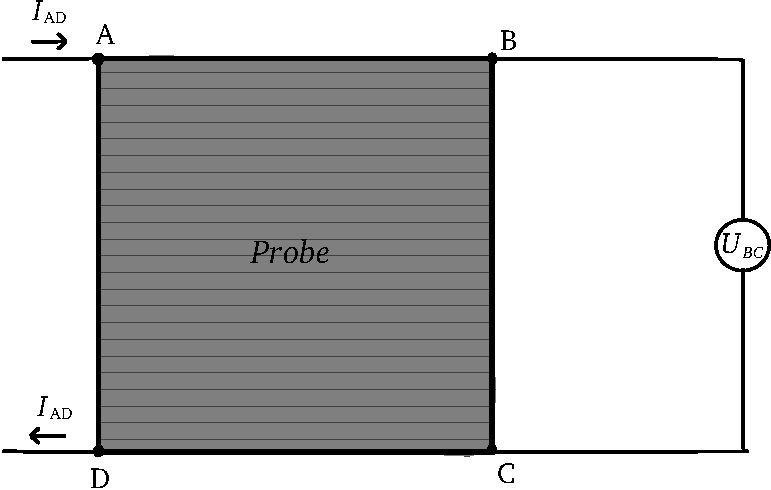
\includegraphics[width=.7\textwidth]{../Abbildungen/Widerstand.pdf}
    \caption{%
        Anschlüsse für die Widerstandsmessung nach van der Pauw
    }
    \label{fig:vdPauw-wid}
\end{figure}

\begin{figure}
    \centering
    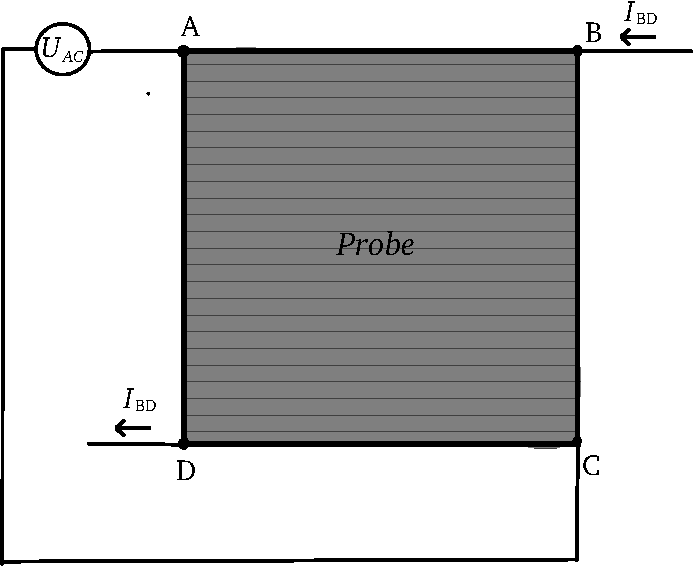
\includegraphics[width=.7\textwidth]{../Abbildungen/Hall-Effekt.pdf}
    \caption{%
        Anschlüsse für die Hall-Effekts-Messung nach van der Pauw
    }
    \label{fig:vdPauw-hall}
\end{figure}

\section{Magnetische Thermospannungen}

\subsection{Seebeck- und Peltier-Effekt}

Liegt in einem (Halb-)Leiter ein Temperaturgradient vor, so ist die Anzahl der
energetisch höher liegenden Elektronen nicht homogen verteilt. Der dadurch
entstehenden Gradient sorgt für einen Stromfluss, der den
Konzentrationsunterschied auszugleichen versucht. Dieser Effekt heißt nach
seinem Entdecker Seebeck-Effekt.

Fließt ein Strom, werden energetisch höher liegende Elektronen transportiert.
Dies sorgt dafür, dass sich diese Elektronen in einem Bereich häufen, was zu
einer Steigerung der Temperatur führt. Dieser umgekehrte Seebeck-Effekt heißt
Peltier-Effekt.

Kombiniert man beide Effekte, sorgt das dafür, dass ein Temperaturgradient
ausgeglichen wird.

\subsection{Ettingshausen- und Nerst-Effekt}

Der Ettingshausen-Effekt wirkt ähnlich wie der Hall-Effekt: Durch die
Ablenkung der Elektronen beim Hall-Effekt, nimmt die Anzahl der Kollisionen in
einem Teil des Leiters zu. Dadurch wird dieser dort erwärmt.

Der Nerst-Effekt ist eine Kombination des Seebeck-Effektes mit dem Hall-Effekt.
Liegt in einem Leiter ein Temperaturgradient senkrecht zu einem angelegten
magnetischen Feld vor, werden die durch den Seebeck-Effekt fließenden
Elektronen wie beim Hall-Effekt abgelenkt. Dabei entsteht ein elektrisches
Feld, bzw. ein senkrecht auf Gradient und Magnetfeld stehende Strom. Dies ist
scheinbar eine Umkehrung des Ettingshausen-Effektes.

Der Nerst- und der Ettingshausen-Effekt werden häufig auch als erster bzw.
zweiter Ettingshausen-Nerst-Effekt bezeichnet.

\subsection{Righi-Leduc-Effekt}

Dieser Effekt, ist das thermische Analogon zum Hall-Effekt. Ein Wärmestrom wird
von einem senkrecht dazu stehenden magnetischen Feld abgelenkt. Dadurch
entsteht hier ein Temperaturgradient.

\FloatBarrier
\chapter{Aufbau}

\FloatBarrier
\chapter{Durchführung}

\section{Widerstandsmessung bei Raumtemperatur}

Zuerst messen wir den Widerstand an den Proben \probeA{} und \probeB. Dazu
benutzen wir die Nummerierung der Schalterstellungen aus
\cite[Tab.~4.1]{heldt/Diplomarbeit}.

Den Strom stellen wir für alle weitere Durchführungen auf $I =
\SI{13.601}{\milli\ampere}$ ein. Dieser hat sich im Laufe des Versuches nur um
\SI{0.01}{\milli\ampere} geändert, so dass dies keine große Fehlerquelle
werden wird.

Die Messungen für die beiden Proben sind in den Tabellen \ref{tab:A:Strom} und
\ref{tab:B:Strom}.

\begin{table}[htbp]
    \centering
    \begin{tabular}{S|SSSSS}
        {Beschaltung} &
        {$U / \si{\milli\volt}$} &
        {$U / \si{\milli\volt}$} &
        {$U / \si{\milli\volt}$} &
        {$U / \si{\milli\volt}$} &
        {$U / \si{\milli\volt}$} \\
        \midrule
        %< for row in messdaten_301_strom: ->%
        << row | join(' & ') >> \\
        %< endfor ->%
    \end{tabular}
    \caption{%
        Gemessene Spannungen bei der Widerstandsmessung für Probe~\probeA. Die
        Wiederholungen der Messung für jede Beschaltung sind jeweils in einer
        Zeile.
    }
    \label{tab:A:Strom}
\end{table}

\begin{table}[htbp]
    \centering
    \begin{tabular}{S|SSSSS}
        {Beschaltung} &
        {$U / \si{\milli\volt}$} &
        {$U / \si{\milli\volt}$} &
        {$U / \si{\milli\volt}$} &
        {$U / \si{\milli\volt}$} &
        {$U / \si{\milli\volt}$} \\
        \midrule
        %< for row in messdaten_540_strom: ->%
        << row | join(' & ') >> \\
        %< endfor ->%
    \end{tabular}
    \caption{%
        Gemessene Spannungen bei der Widerstandsmessung für Probe~\probeB. Die
        Wiederholungen der Messung für jede Beschaltung sind jeweils in einer
        Zeile.
    }
    \label{tab:B:Strom}
\end{table}

\section{Messung der Hallkonstanten bei Raumtemperatur}

Für die Messung der Hallkonstanten an den beiden Proben benutzen wir den
Permanentmagneten mit $B = \SI{0.138 +-
0.001}{\tesla}$\footnote{\erklaerungFehlerNotation}.

Die Messdaten sind in den Tabellen \ref{tab:A:Hall} und \ref{tab:B:Hall}.

\begin{table}[htbp]
    \centering
    \begin{tabular}{S|SSSSS}
        {Beschaltung} &
        {$U / \si{\milli\volt}$} &
        {$U / \si{\milli\volt}$} &
        {$U / \si{\milli\volt}$} &
        {$U / \si{\milli\volt}$} &
        {$U / \si{\milli\volt}$} \\
        \midrule
        %< for row in messdaten_301_hall: ->%
        << row | join(' & ') >> \\
        %< endfor ->%
    \end{tabular}
    \caption{%
        Gemessene Spannungen bei der Messung der Hallkonstanten für
        Probe~\probeA. Die Wiederholungen der Messung für jede Beschaltung ist
        jeweils in einer Zeile.
    }
    \label{tab:A:Hall}
\end{table}

\begin{table}[htbp]
    \centering
    \begin{tabular}{S|SSSSS}
        {Beschaltung} &
        {$U / \si{\milli\volt}$} &
        {$U / \si{\milli\volt}$} &
        {$U / \si{\milli\volt}$} &
        {$U / \si{\milli\volt}$} &
        {$U / \si{\milli\volt}$} \\
        \midrule
        %< for row in messdaten_540_hall: ->%
        << row | join(' & ') >> \\
        %< endfor ->%
    \end{tabular}
    \caption{%
        Gemessene Spannungen bei der Messung der Hallkonstanten für
        Probe~\probeB. Die Wiederholungen der Messung für jede Beschaltung ist
        jeweils in einer Zeile.
    }
    \label{tab:B:Hall}
\end{table}

\section{Messungen bei verschiedenen Temperaturen}

Nach Beendigung der letzten Messung an Probe~\probeB{} lassen wir diese im
Kryostaten und starten die Kühlung. Am nächsten Tag fahren wir mit der Messung
bei der niedrigsten Temperatur fort. Wir heizen für jede weitere Messreihe die
Probe mit den Heizwiderständen auf und halten die Temperatur dann möglichst
konstant. Die Schwankung, die wir während den Messreihen beobachtet haben,
haben wir als Fehler angegeben.

Bei jeder Temperatur haben wir eine Messreihe für den Widerstand und eine für
die Hallkonstante vorgenommen. Die Ergebnisse sind in Tabelle
\ref{tab:Strom_Temp} bzw. \ref{tab:Hall_Temp}. Bei der Temperatur handelt es
sich um die mit der ausliegenden Tabelle konvertierte Thermospannung. Erst in
der Auswertung korrigieren wir die Verschiebung durch die erhöhte
Raumtemperatur.

\begin{landscape}
    \begin{table}[htbp]
        \centering
        \begin{tabular}{SS|SSSSSSSS}
            {$T/ \si\celsius$}
            & {$T_\text{Raum} / \si\celsius$}
            %< for header in range(1, 9): ->%
            & {$U_{<< header >>}$}
            %< endfor ->%
            \\
            \midrule
            %< for row in messdaten_temp_strom: ->%
            << row | join(' & ') >> \\
            %< endfor ->%
        \end{tabular}
        \caption{%
            Gemessene Spannungen (in \si{\milli\volt}) bei der Messung des
            Widerstands für Probe~\probeB{} bei verschiedenen Temperaturen. In
            den Spalten stehen die verschiedenen Beschaltungen, in den Zeilen
            die unterschiedlichen Temperaturen.
        }
        \label{tab:Strom_Temp}
    \end{table}
\end{landscape}

\begin{landscape}
    \begin{table}[htbp]
        \centering
        \begin{tabular}{SS|SSSSSSSSSS}
            {$T/ \si\celsius$}
            & {$T_\text{Raum} / \si\celsius$}
            %< for header in range(1, 11): ->%
            & {$U_{<< header >>}$}
            %< endfor ->%
            \\
            \midrule
            %< for row in messdaten_temp_hall: ->%
            << row | join(' & ') >> \\
            %< endfor ->%
        \end{tabular}
        \caption{%
            Gemessene Spannungen (in \si{\milli\volt}) bei der Messung der
            Hallkonstanten für Probe~\probeB{} bei verschiedenen Temperaturen.
            In den Spalten stehen die verschiedenen Beschaltungen, in den
            Zeilen die unterschiedlichen Temperaturen.
        }
        \label{tab:Hall_Temp}
    \end{table}
\end{landscape}

\chapter{Auswertung}

\section{Bestimmung des spezifischen Widerstands bei Raumtemperatur}
\label{sec:spez-wid-rt}

Aus den gemessenen Spannungen bestimmen wir nach \cite{heldt/Diplomarbeit}
mit dem eingestellten Strom Widerstände. Die gemessenen 8 Spannungen, die wir
wie in \cite[Tab.~4.1]{heldt/Diplomarbeit}, $V_1$ bis $V_8$ nennen werden,
werden wie folgt verrechnet:
\[
    R_{ij,kl} := \frac{|V_i - V_j|}{2 I_{kl}} = \frac{|V_i - V_j|}{2 I}.
\]

Dabei ist $I_{kl} = I$, da wir den Strom während der ganzen Durchführung auf
dem Wert $I = \SI{<< I_mA >>}{\milli\ampere}$ eingestellt haben. Die
Zwischenergebnisse sind in den Tabellen \ref{tab:A:R} und \ref{tab:B:R}
gezeigt.

\begin{table}[htbp]
    \centering
    \begin{tabular}{SSSS|SS}
        {$R_{1234} / \si\ohm$} &
        {$R_{2341} / \si\ohm$} &
        {$R_{3412} / \si\ohm$} &
        {$R_{4132} / \si\ohm$} &
        {$R_{1234} / R_{2341}$} &
        {$R_{3412} / R_{4121}$} \\
        \midrule
        %< for row in hf_540_strom_R_tabelle: ->%
        << row | join(' & ') >> \\
        %< endfor ->%
    \end{tabular}
    \caption{%
        Widerstände für die Probe \probeA.
    }
    \label{tab:A:R}
\end{table}

\begin{table}[htbp]
    \centering
    \begin{tabular}{SSSS|SS}
        {$R_{1234} / \si\ohm$} &
        {$R_{2341} / \si\ohm$} &
        {$R_{3412} / \si\ohm$} &
        {$R_{4132} / \si\ohm$} &
        {$R_{1234} / R_{2341}$} &
        {$R_{3412} / R_{4121}$} \\
        \midrule
        %< for row in hf_301_strom_R_tabelle: ->%
        << row | join(' & ') >> \\
        %< endfor ->%
    \end{tabular}
    \caption{%
        Widerstände für die Probe \probeB.
    }
    \label{tab:B:R}
\end{table}

Aus je zwei Widerständen können wir dann nach der van der Pauw-Methode einen
Wert für den spezifischen Widerstand bestimmen \parencite[Formel (4.9) und
(4.10)]{heldt/Diplomarbeit}:
\begin{align*}
    \rho_1 &= \frac{\piup d}{\ln(2)} \frac{R_{12,34} + R_{23,41}}{2}
    \, f\del{\frac{R_{12,34}}{R_{23,41}}} \\
    %
    \rho_2 &= \frac{\piup d}{\ln(2)} \frac{R_{34,12} + R_{41.23}}{2}
    \, f\del{\frac{R_{34,12}}{R_{41.23}}}.
\end{align*}

Dabei ist $f$ ein Korrekturfaktor für die Assymetrie der Probe. Aus
\cite[Abb.~4.4]{heldt/Diplomarbeit}, können wir diesen Korrekturfaktor ablesen.
Wie in Tabellen \ref{tab:A:R} und \ref{tab:B:R} zu sehen ist, sind die
Verhältnisse der $R_{ij,kl}$ derart nahe bei 1, dass wir $f = 1$ annehmen
können.

Aus den beiden Werten für den spezifischen Widerstand bilden wir den
Mittelwert und erhalten für jede der fünf Messreihen einen Wert für $\rho$.
Diese Ergebnisse sind in den Tabellen \ref{tab:A:rho} und \ref{tab:B:rho}
abgedruckt.

\begin{table}[htbp]
    \centering
    \begin{tabular}{SS|S}
        {$\rho_1 d^{-1} / \si\ohm$} &
        {$\rho_2 d^{-1} / \si\ohm$} &
        {$\rho d^{-1} / \si\ohm$} \\
        \midrule
        %< for row in hf_540_strom_rho_tabelle: ->%
        << row | join(' & ') >> \\
        %< endfor ->%
    \end{tabular}
    \caption{%
        Spezifische Widerstände für die Probe \probeA.
    }
    \label{tab:A:rho}
\end{table}

\begin{table}[htbp]
    \centering
    \begin{tabular}{SS|S}
        {$\rho_1 d^{-1} / \si\ohm$} &
        {$\rho_2 d^{-1} / \si\ohm$} &
        {$\rho d^{-1} / \si\ohm$} \\
        \midrule
        %< for row in hf_301_strom_rho_tabelle: ->%
        << row | join(' & ') >> \\
        %< endfor ->%
    \end{tabular}
    \caption{%
        Spezifische Widerstände für die Probe \probeB.
    }
    \label{tab:B:rho}
\end{table}

Diese fünf Werte pro Probe mitteln wir zu einem endgültigen Ergebnis. Den
Fehler bestimmen wir mit der Standardabweichung, die wir im folgenden mit dem
Operator $\std$ bezeichnen werden. Somit erhalten wir also:
\[
    \rho = \bracket{\{\rho\}}
    \eqnsep
    \Deltaup \rho = \std(\{\rho\})
\]

Für die Proben \probeA{} und \probeB{} erhalten wir so $\rho d^{-1} = \SI{<<
hf_540_strom_rho >>}{\ohm}$ bzw. $\rho d^{-1} = \SI{<< hf_301_strom_rho
>>}{\ohm}$ aus allen fünf Messreihen.

Da nach der Leitfähigkeit gefragt ist, rechnen wir $\rho d^{-1}$ um. Den Fehler
erhalten wir nach Gauß'scher Fehlerfortplanzung. Wir erhalten $\sigma d =
\SI{<< hf_540_strom_sigma >>}{\per\kilo\ohm}$ bzw. $\sigma d = \SI{<<
hf_301_strom_sigma >>}{\per\kilo\ohm}$.

\section{Bestimmung der Hallkonstanten bei Raumtemperatur}
\label{sec:hall-rt}

Die Bestimmung der Hallkonstanten ähnelt in einigen Schritten der vorherigen
Bestimmung des spezifischen Widerstands. Die 10 Spannungen, die wir gemessen
haben, nennen wir wieder $V_1$ bis $V_{10}$
\parencite[Tab.~4.2]{heldt/Diplomarbeit}.

Es gibt zwei Methoden, aus einer Teilmenge dieser 10 Spannungen die
Hallkonstante zu bestimmen. Wir werden hier beide durchführen, angefangen mit
der Methode, die die Messungen ohne magnetische Induktion, $V_9$ und $V_{10}$,
einbeziehen.

\subsection{Mit Nullfeldmessung}

Aus den 10 Messungen werden 6 ausgewählt. Diese werden wie folgt verrechnet
\parencite[Formel (4.14) und (4.15)]{heldt/Diplomarbeit}:
\begin{align*}
    V_{\text H+} &= \half\del[1]{(\overbrace{V_1 - V_9}^{\Deltaup V_\text A}) - (\overbrace{V_2 - V_{10}}^{\Deltaup V_\text B})} \\
    V_{\text H-} &= - \half\del[1]{(\underbrace{V_5 - V_9}_{\Deltaup V_\text C}) - (\underbrace{V_6 - V_{10}}_{\Deltaup V_\text D})}.
\end{align*}

Die Zwischenergebnisse sind in den Tabellen \ref{tab:A:V_ABCD} und
\ref{tab:B:V_ABCD} aufgelistet. Die Hallspannungen und -konstanten für beide
Magnetfeldrichtungen sind in den Tabellen \ref{tab:A:VH+-,RH+-} und
\ref{tab:B:VH+-,RH+-} aufgelistet.

\begin{table}[htbp]
    \centering
    \begin{tabular}{SSSS}
        {$\Deltaup V_\text{A} / \si{\milli\volt}$} &
        {$\Deltaup V_\text{B} / \si{\milli\volt}$} &
        {$\Deltaup V_\text{C} / \si{\milli\volt}$} &
        {$\Deltaup V_\text{D} / \si{\milli\volt}$} \\
        \midrule
        %< for row in hf_540_hall_V_tabelle_mV: ->%
        << row | join(' & ') >> \\
        %< endfor ->%
    \end{tabular}
    \caption{%
        Spannungsdifferenzen bei der Messung der Hallkonstanten für die Probe
        \probeA.
    }
    \label{tab:A:V_ABCD}
\end{table}

\begin{table}[htbp]
    \centering
    \begin{tabular}{SSSS}
        {$\Deltaup V_\text{A} / \si{\milli\volt}$} &
        {$\Deltaup V_\text{B} / \si{\milli\volt}$} &
        {$\Deltaup V_\text{C} / \si{\milli\volt}$} &
        {$\Deltaup V_\text{D} / \si{\milli\volt}$} \\
        \midrule
        %< for row in hf_301_hall_V_tabelle_mV: ->%
        << row | join(' & ') >> \\
        %< endfor ->%
    \end{tabular}
    \caption{%
        Spannungsdifferenzen bei der Messung der Hallkonstanten für die Probe
        \probeB.
    }
    \label{tab:B:V_ABCD}
\end{table}

\begin{table}[htbp]
    \centering
    \begin{tabular}{SS|SS}
        {$V_{H+} / \si\volt$} &
        {$V_{H-} / \si\volt$} &
        {$R_{H+} d^{-1} / \si{\volt\per\tesla\per\ampere}$} &
        {$R_{H-} d^{-1} / \si{\volt\per\tesla\per\ampere}$} \\
        \midrule
        %< for row in hf_540_hall_V_R_tabelle: ->%
        << row | join(' & ') >> \\
        %< endfor ->%
    \end{tabular}
    \caption{%
        Hallkonstanten für die Probe \probeA.
    }
    \label{tab:A:VH+-,RH+-}
\end{table}

\begin{table}[htbp]
    \centering
    \begin{tabular}{SSSS}
        {$V_{H+} / \si{\milli\volt}$} &
        {$V_{H-} / \si{\milli\volt}$} &
        {$R_{H+} d^{-1} / \si{\volt\per\tesla\per\ampere}$} &
        {$R_{H-} d^{-1} / \si{\volt\per\tesla\per\ampere}$} \\
        \midrule
        %< for row in hf_301_hall_V_R_tabelle: ->%
        << row | join(' & ') >> \\
        %< endfor ->%
    \end{tabular}
    \caption{%
        Hallkonstanten für die Probe \probeB.
    }
    \label{tab:B:VH+-,RH+-}
\end{table}

Wir bilden wie im vorherigen Teil Mittelwert und Fehler. Wir erhalten so für
Proble \probeA{} $R_{H+} = \SI{<< hf_540_hall_R_H_plus
>>}{\volt\per\tesla\per\ampere}$ und $R_{H-} = \SI{<< hf_540_hall_R_H_minus
>>}{\volt\per\tesla\per\ampere}$ aus allen fünf Messreihen.

Bei Probe \probeB{} sind die Werte $R_{H+} = \SI{<< hf_301_hall_R_H_plus
>>}{\volt\per\tesla\per\ampere}$ und $R_{H-} = \SI{<< hf_301_hall_R_H_minus
>>}{\volt\per\tesla\per\ampere}$.

\subsection{Ohne Nullfeldmessung}

Es ist auch möglich, die ersten 8 Messwerte (die mit angelegter magnetischer
Flussdichte) so zu verrechnen, dass keine Nullfeldmessung notwendig ist. Dazu
werden zwei Zwischenwerte berechnet \parencite[Formel (4.18) und
(4.19)]{heldt/Diplomarbeit}:
\begin{align*}
    R_{\text H1} d^{-1} &= \frac{1}{BI} \frac{(V_1 - V_2) - (V_5 - V_6)}{4} \\
    R_{\text H2} d^{-1} &= \frac{1}{BI} \frac{(V_3 - V_4) - (V_7 - V_8)}{4}.
\end{align*}

Aus den beiden Hallkonstanten pro Messreihe wird der Mittelwert genommen und
wir erhalten eine Hallkonstante pro Messreihe. Diese drei Werte sind für die
beiden Proben in den Tabellen \ref{tab:A:H_12} und \ref{tab:B:H_12} aufgeführt.

\begin{table}[htbp]
    \centering
    \begin{tabular}{SS|S}
        {$R_{H1} d^{-1} / \si{\volt\per\tesla\per\ampere}$} &
        {$R_{H2} d^{-1} / \si{\volt\per\tesla\per\ampere}$} &
        {$R_{H} d^{-1} / \si{\volt\per\tesla\per\ampere}$} \\
        \midrule
        %< for row in hf_540_hall_RH_mit_tabelle: ->%
        << row | join(' & ') >> \\
        %< endfor ->%
    \end{tabular}
    \caption{%
        Hallkonstanten für die Probe \probeA, nach der Auswertungsmethode ohne
        Nullmessung.
    }
    \label{tab:A:H_12}
\end{table}

\begin{table}[htbp]
    \centering
    \begin{tabular}{SS|S}
        {$R_{H1} d^{-1} / \si{\volt\per\tesla\per\ampere}$} &
        {$R_{H2} d^{-1} / \si{\volt\per\tesla\per\ampere}$} &
        {$R_{H} d^{-1} / \si{\volt\per\tesla\per\ampere}$} \\
        \midrule
        %< for row in hf_301_hall_RH_mit_tabelle: ->%
        << row | join(' & ') >> \\
        %< endfor ->%
    \end{tabular}
    \caption{%
        Hallkonstanten für die Probe \probeB, nach der Auswertungsmethode ohne
        Nullmessung.
    }
    \label{tab:B:H_12}
\end{table}

Wir bilden Mittelwert und Fehler und erhalten so $R_{H} = \SI{<<
hf_540_hall_R_H >>}{\volt\per\tesla\per\ampere}$ und $R_{H} = \SI{<<
hf_301_hall_R_H >>}{\volt\per\tesla\per\ampere}$ aus allen fünf Messreihen für
Probe \probeA{} bzw. Probe \probeB{}.

\section{Bestimmung der Beweglichkeit und Ladungsträgerdichte}

Aus den bisher errechneten Größen $\sigma$ und $R_\text H$ errechnen wir nun
die Beweglichkeit $\mu$ und die Ladungsträgerdichte der Majoritätsladung $p$:
\[
    p = \frac1{e R_\text H}
    \eqnsep
    \mu = \abs{\frac{R_\text H}{\rho}}
\]

Die so errechneten Größen sind in Tabelle~\ref{tab:mu-p}.

\begin{table}[htbp]
    \centering
    \begin{tabular}{lSSS}
        Probe &
        {$\sigma d / \si{\per\kilo\ohm}$} &
        {$\mu_{\text H} d^{-1} / \si{\ohm\volt\per\tesla\per\ampere}$} &
        {$p d / \SI{e15}{\per\square\meter}$} \\
        \midrule
        %< for row in zimmertemperatur_tabelle1: ->%
        << row | join(' & ') >> \\
        %< endfor ->%
    \end{tabular}
    \caption{%
        Errechnete Beweglichkeiten und Ladungsträgerdichten
    }
    \label{tab:mu-p}
\end{table}

\section{Untersuchung der Temperaturabhängigkeit}

Die Auswertungsmethoden, die wir in für die Messungen bei Raumtemperatur
benutzt haben, nutzen wir hier ebenfalls aus. Da wir jedoch nur eine Messreihe
pro Temperatur haben, entfällt hier die Mittelwertbildung. 

Die direkt vor Ort in eine Temperatur in \si{\celsius} umgerechneten
Thermospannungen haben wir hier in der Auswertung noch um die Verschiebung
$\SI{5}\kelvin$ angepasst, die wir durch die erhöhte Raumtemperatur von
\SI{25}{\celsius} hatten. Außerdem haben wir die Temperaturen in Kelvin
umgerechnet.

Alle Werte sind in Tabelle~\ref{tab:Temperaturabhängigkeit} zusammengestellt.

\begin{table}[htbp]
    \centering
    \begin{tabular}{SSSSS}
        {$T / \si\kelvin$} &
        {$\sigma d / \si{\kilo\ohm}$} &
        {$R_\text H d^{-1}$} &
        {$p d^{-1} / \SI{e15}{\per\cubic\meter}$} &
        {$\mu d^{-1}$} \\
        \midrule
        %< for row in temperatur_tabelle: ->%
        << row | join(' & ') >> \\
        %< endfor ->%
    \end{tabular}
    \caption{%
    }
    \label{tab:Temperaturabhängigkeit}
\end{table}

In Abbildung~\ref{fig:sigma-T} ist die Abhängigkeit der Leitfähigkeit von der
Temperatur dargestellt. Für große $T$, also kleine $T^{-1}$ sinkt die
Leitfähigkeit.

\begin{figure}[htbp]
    \centering
    \includegraphics[width=\linewidth]{plot1.pdf}
    \caption{%
        Zusammenhang zwischen Leitfähigkeit und Temperatur.
    }
    \label{fig:sigma-T}
\end{figure}

Der Graph in Abbildung~\ref{fig:p-T} zeigt den Zusammenhang zwischen der
Ladungsträgerdichte und Temperatur. Für große $T$ steigt die
Ladungsträgerdichte. Davor gibt es noch ein Minimum.

\fehlt

\begin{figure}[htbp]
    \centering
    \includegraphics[width=\linewidth]{plot2.pdf}
    \caption{%
    }
    \label{fig:p-T}
\end{figure}

\begin{figure}[htbp]
    \centering
    \includegraphics[width=\linewidth]{plot3.pdf}
    \caption{%
    }
    \label{fig:}
\end{figure}

\chapter{Diskussion}

In Tabelle~\ref{tab:zimmertemperatur_tabelle1} haben wir die endgültigen Werte
für $\sigma$ zusammengetragen und $\mu_\text H$ sowie $p$ berechnet. In
Tabelle~\ref{tab:zimmertemperatur_tabelle2} sind die Hallkonstanten
zusammengefasst.

\begin{table}[htbp]
    \centering
    \begin{tabular}{lSSS}
        Probe &
        {$\sigma d / \si{\per\kilo\ohm}$} &
        {$\mu_{\text H} d^{-1} / \si{\ohm\volt\per\tesla\per\ampere}$} &
        {$p / \SI{e15}{\per\cubic\meter}$} \\
        \midrule
        %< for row in zimmertemperatur_tabelle1: ->%
        << row | join(' & ') >> \\
        %< endfor ->%
    \end{tabular}
    \caption{%
        Zusammenstellung der Ergebnisse aus dem ersten Versuchsteil, Teil~1.
    }
    \label{tab:zimmertemperatur_tabelle1}
\end{table}

\begin{table}[htbp]
    \centering
    \begin{tabular}{lSSS}
        Probe &
        {$R_{\text H+} d^{-1} / \si{\volt\per\tesla\per\ampere}$} &
        {$R_{\text H-} d^{-1} / \si{\volt\per\tesla\per\ampere}$} &
        {$R_{\text H} d^{-1} / \si{\volt\per\tesla\per\ampere}$} \\
        \midrule
        %< for row in zimmertemperatur_tabelle2: ->%
        << row | join(' & ') >> \\
        %< endfor ->%
    \end{tabular}
    \caption{%
        Zusammenstellung der Ergebnisse aus dem ersten Versuchsteil, Teil~2.
    }
    \label{tab:zimmertemperatur_tabelle2}
\end{table}

Es fällt auf, dass die Leitfähigkeiten recht nahe beiander
liegen. Die Hallkonstanten liegen betragsmäßig ebenfalls recht nahe
beieinander, unterscheiden sich jedoch im Vorzeichen.

In beiden Fällen ist $R_\text H$ innerhalb des Fehlerbereichs der Mittelwert
auf $R_{\text H+}$ und $R_{\text H-}$. Dies bedeutet, dass beide Mess- und
Auswertungsmethoden das Nullfeld gleich korrigieren.

Aus der Ladungsträgerkonzentration (siehe
Tabelle~\ref{tab:zimmertemperatur_tabelle1}), die für positive Ladungsträger
berechnet worden ist, folgt, dass die Probe~\probeA{} negativ und die
Probe~\probeB{} positiv dotiert ist.

\printbibliography

\end{document}

% vim: et spell spelllang=de tw=79
